\documentclass{beamer}
\usetheme{Madrid}

\usepackage{amsmath, amssymb, amsthm}
\usepackage{graphicx}
\usepackage{listings}
\usepackage{physics}
\usepackage{gensymb}
\usepackage[utf8]{inputenc}
\usepackage{hyperref}
\usepackage{tikz}
\lstset{
%language=C,
frame=single, 
breaklines=true,
columns=fullflexible
}
\usetikzlibrary{decorations.pathmorphing}

\title{Question-7-7.2-8}
\author{EE24BTECH11033 - K.SURAJ}
\date{}
\begin{document}

\frame{\titlepage}
\begin{frame}
\frametitle{Question}
The centre of circle is $\begin{pmatrix}2a\\a-7\end{pmatrix}$. Find the values of $a$ if the circle passes through the point $\vec{A}\begin{pmatrix}11\\-9\end{pmatrix}$ and has diameter $10\sqrt{2}$ units.
\end{frame}
\begin{frame}
\frametitle{Inputs}

  \centering
\begin{tabular}{ |c| c|}
    \hline
    \textbf{Description}  & \textbf{ Given value}\\
    \hline
    Centre  & $\begin{pmatrix}2a\\a-7\end{pmatrix}$\\
    \hline
    Diameter & $10\sqrt{2}$\\
    \hline
    point $\vec{A}$ & $\begin{pmatrix}11\\-9\end{pmatrix}$\\
    \hline
\end{tabular}


    
\end{frame}
\begin{frame}{Formulas}
    \centering
\begin{tabular}{ |c|c|}
    \hline
    \textbf{Conic} & \textbf{Expression}\\ 
    \hline
    Circle & $\norm{\vec{x}}^2 + 2 \vec{u}^\top\vec{x} + f = 0$ \\
    \hline
   
\end{tabular}
\end{frame}

\begin{frame}{Solution}


        The radius of circle is $\frac{diameter}{2}$
\begin{align*}
    \implies radius=5\sqrt{2}
    \end{align*}
     The equation of a circle is given by 
	
\begin{align}
	\norm{\vec{x}}^2 + 2 \vec{u}^{\top}\vec{x} + f = 0\label{5}
\end{align}
for
		\begin{align}
	 \vec{u}=-\vec{c}, f = \norm{\vec{c}}^2-r^2
		\end{align}
  Where $\vec{c}$ is centre and $r$ is the radius of the circle
\end{frame}
\begin{frame}{Solution}
    Now,
  \begin{align}
      \vec{u}=-\begin{pmatrix}2a\\a-7\end{pmatrix},f=5a^2-14a-1
  \end{align}
  On substituting $x$=$\begin{pmatrix}11\\-9\end{pmatrix}$ in (\ref{5}) We get, \\
  \begin{align*}
  202-26a-126+5a^2-14a-1=0\\
  5a^2-40a+75=0\\
  a^2-8a+15=0\\
  a=3,a=5
  \end{align*}
\end{frame}


\section{C Code}
\begin{frame}[fragile]
\frametitle{C Code}
\begin{lstlisting}[language=C]
#include <stdio.h>
#include <stdlib.h>
#include <string.h>
#include <math.h>
#include <unistd.h>
#include "libs/matfun.h"
#include "libs/geofun.h"

void point_gen(FILE *fptr, double **A, double **B, int no_rows, int no_cols, int num_points) {
    for (int i = 0; i < num_points; i++) {
        double t = (double)i / (num_points - 1);
        double **output = Matadd(A, Matscale(Matsub(B, A, no_rows, no_cols), no_rows, no_cols, t), no_rows, no_cols);
        fprintf(fptr, "%lf,%lf\n", output[0][0], output[1][0]);
        freeMat(output, no_rows);}}
\end{lstlisting}
\end{frame}
\begin{frame}[fragile]
\frametitle{C Code}
\begin{lstlisting}[language=C]
double** centre_gen(double x1, double x2, double y1, double y2, double **ptA, double diameter){
    double m = y1/x1;
    double c = y2-m*x2; 
    double radius = diameter/2;
    double A=(1+m*m);
    double B=(2*m*(c-ptA[1][0])-2*ptA[0][0]);
    double C=(ptA[0][0]*ptA[0][0])+((ptA[1][0]-c)*(ptA[1][0]-c)) - (radius*radius);
    double** points = createMat(2,2);
    points[0][0] = (-B+sqrt(B*B-4*A*C))/(2*A);
    points[1][0] = m*points[0][0]+c;
    points[0][1] = (-B-sqrt(B*B-4*A*C))/(2*A);
    points[1][1] = m*points[0][1]+c;
    return points;
}
\end{lstlisting}
\end{frame}
\begin{frame}[fragile]
\frametitle{C Code}
\begin{lstlisting}[language=C]
void circle_point_gen(FILE *fptr, double radius, double **center, int num_points) {
    double **output;
    for (int i = 0; i <= num_points; i++) {
        double angle = (2 * M_PI * i) / num_points;
        output = createMat(2, 1);
        output[0][0] = center[0][0] + radius * cos(angle);
        output[1][0] = center[1][0] + radius * sin(angle);
        fprintf(fptr, "%lf,%lf\n", output[0][0], output[1][0]);
        freeMat(output, 2);
    }
}
\end{lstlisting}
\end{frame}
\begin{frame}[fragile]
\frametitle{C Code}
\begin{lstlisting}[language=C]
int main() {
    double a = 1.0; //for graphing
    double** A = createMat(2,1);
    A[0][0] = 11;
    A[1][0] = -9;
    double diameter = 10*sqrt(2); 
    double** centers = centre_gen(2,0,1,-7,A,diameter);
    double** center1 = createMat(2,1);
    double** center2 = createMat(2,1);
    center1[0][0] = centers[0][0];
    center1[1][0] = centers[1][0];
    center2[0][0] = centers[0][1];
    center2[1][0] = centers[1][1];
    printMat(center1,2,1);
    printMat(center2,2,1);
    printf("%lf",diameter/2);
\end{lstlisting}
\end{frame}
\begin{frame}[fragile]
\frametitle{C Code}
\begin{lstlisting}[language=C]
 FILE *fptr = fopen("points.dat", "w");
    if (fptr == NULL) {
        printf("Error opening file!\n");
        return 1;
    }
    
    circle_point_gen(fptr, diameter/2, center1, 100);
    circle_point_gen(fptr, diameter/2, center2, 100);

    fclose(fptr);
    return 0;
}
\end{lstlisting}
\end{frame}
\section{Python Code}
\begin{frame}[fragile]
\frametitle{Python Code for Plotting}
\begin{lstlisting}[language=Python]
import numpy as np
import matplotlib.pyplot as plt

# Load points from the data file
points = np.loadtxt("points.dat", delimiter=',')
x_circle1 = points[:101, 0]
y_circle1 = points[:101, 1]
x_circle2 = points[101:, 0]
y_circle2 = points[101:, 1]

# Circle 1 center and radius
center1 = ((x_circle1[0]+x_circle1[50])/2, (y_circle1[0]+y_circle1[50])/2)
radius1 = np.sqrt((x_circle1[0] - center1[0])**2 + (y_circle1[0] - center1[1])**2)
circle_eq1 = f'(x-{center1[0]:.2f})^2 + (y-{center1[1]:.2f})^2 = {radius1**2:.2f}'

\end{lstlisting}
\end{frame}
\begin{frame}[fragile]
\frametitle{Python Code for Plotting}
\begin{lstlisting}[language=Python]
center2 = ((x_circle2[0]+x_circle2[50])/2, (y_circle2[0]+y_circle2[50])/2)
radius2 = np.sqrt((x_circle2[0] - center2[0])**2 + (y_circle2[0] - center2[1])**2)
circle_eq2 = f'(x-{center2[0]:.2f})^2 + (y-{center2[1]:.2f})^2 = {radius2**2:.2f}'

# Create subplots
fig, axes = plt.subplots(1, 2, figsize=(12, 6))

\end{lstlisting}
\end{frame}
\begin{frame}[fragile]
\frametitle{Python Code for Plotting}
\begin{lstlisting}[language=Python]
# Plot the first circle in the first subplot
axes[0].plot(x_circle1, y_circle1, label='Circle 1', color='orange')
axes[0].fill(x_circle1, y_circle1, 'lightblue', alpha=0.5)
axes[0].scatter(*center1, color='red', label='Center 1')
axes[0].text(center1[0], center1[1], f'({center1[0]:.2f}, {center1[1]:.2f})', fontsize=10, ha='right')
axes[0].text(center1[0], center1[1] + radius1, circle_eq1, fontsize=12, ha='center', color='black')
axes[0].set_title("Circle 1")
axes[0].set_xlabel("x")
axes[0].set_ylabel("y")
axes[0].axis('equal')
axes[0].grid(True)
axes[0].legend(loc="upper right")
\end{lstlisting}
\end{frame}
\begin{frame}[fragile]
\frametitle{Python Code for Plotting}
\begin{lstlisting}[language=Python]
# Plot the second circle in the second subplot
axes[1].plot(x_circle2, y_circle2, label='Circle 2', color='green')
axes[1].fill(x_circle2, y_circle2, 'lightgreen', alpha=0.5)
axes[1].scatter(*center2, color='red', label='Center 2')
axes[1].text(center2[0], center2[1], f'({center2[0]:.2f}, {center2[1]:.2f})', fontsize=10, ha='right')
axes[1].text(center2[0], center2[1] + radius2, circle_eq2, fontsize=12, ha='center', color='black')
axes[1].set_title("Circle 2")
axes[1].set_xlabel("x")
axes[1].set_ylabel("y")
axes[1].axis('equal')
axes[1].grid(True)
axes[1].legend(loc="upper right")
\end{lstlisting}
\end{frame}
\begin{frame}[fragile]
\frametitle{Python Code for Plotting}
\begin{lstlisting}[language=Python]
# Adjust layout and save the plot
plt.tight_layout()
plt.savefig('../figs/Figure_1.png')
\end{lstlisting}
\end{frame}
\begin{frame}{Diagram}
\begin{figure}[!ht]
    \centering
    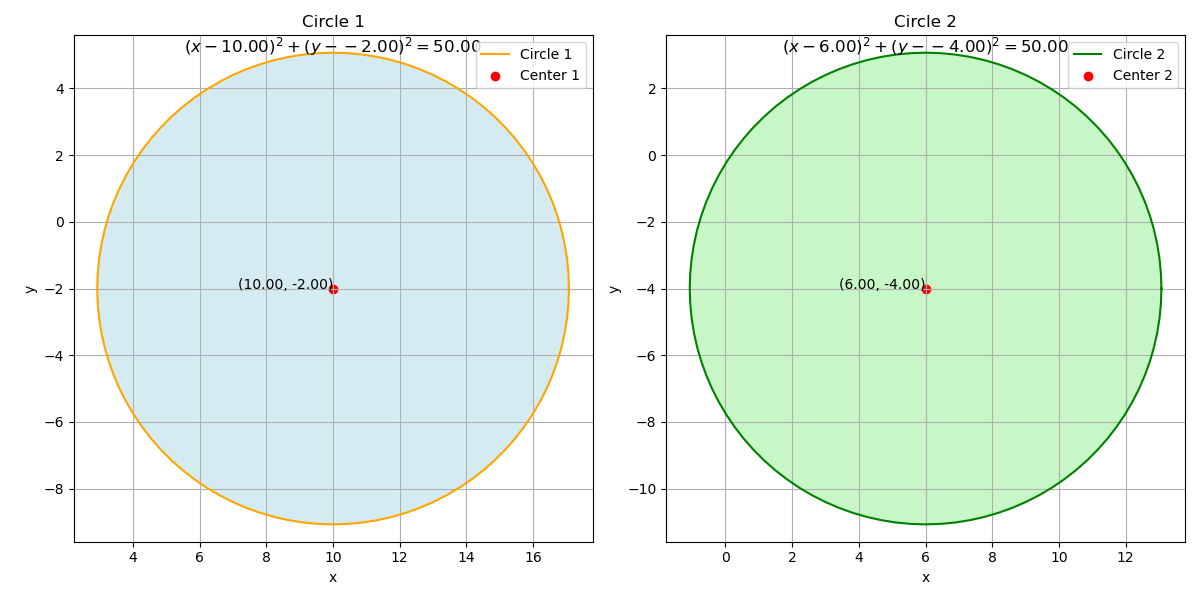
\includegraphics[width=\linewidth]{figs/Figure_1.png}
    
\end{figure}
    
\end{frame}




































\end{document}
